\documentclass[review, times]{elsarticle}

\usepackage{lineno,hyperref}
\modulolinenumbers[5]

\journal{Journal of \LaTeX\ Templates}

%%%%%%%%%%%%%%%%%%%%%%%
%% Elsevier bibliography styles
%%%%%%%%%%%%%%%%%%%%%%%
%% To change the style, put a % in front of the second line of the current style and
%% remove the % from the second line of the style you would like to use.
%%%%%%%%%%%%%%%%%%%%%%%

%% Numbered
%\bibliographystyle{model1-num-names}

%% Numbered without titles
%\bibliographystyle{model1a-num-names}

%% Harvard
%\bibliographystyle{model2-names.bst}\biboptions{authoryear}

%% Vancouver numbered
%\usepackage{numcompress}\bibliographystyle{model3-num-names}

%% Vancouver name/year
%\usepackage{numcompress}\bibliographystyle{model4-names}\biboptions{authoryear}

%% APA style
%\bibliographystyle{model5-names}\biboptions{authoryear}

%% AMA style
%\usepackage{numcompress}\bibliographystyle{model6-num-names}

%% `Elsevier LaTeX' style
\bibliographystyle{elsarticle-num}
%%%%%%%%%%%%%%%%%%%%%%%


% personal packages
\usepackage{amsmath,amssymb}
\usepackage{subfig}
\usepackage{tabu}
\usepackage{booktabs}


% personal macros
\newcommand*\diff{\mathop{}\!\mathrm{d}}
\newcommand*\Diff[1]{\mathop{}\!\mathrm{d^#1}}

\begin{document}

\begin{frontmatter}

\title{A fast spectral method for inelastic collision operator and the heated granular flow\tnoteref{mytitlenote}}
\tnotetext[mytitlenote]{Fully documented templates are available in the elsarticle package on \href{http://www.ctan.org/tex-archive/macros/latex/contrib/elsarticle}{CTAN}.}

%% Group authors per affiliation:
\author{Elsevier\fnref{myfootnote}}
\address{Radarweg 29, Amsterdam}
\fntext[myfootnote]{Since 1880.}

%% or include affiliations in footnotes:
\author[mymainaddress,mysecondaryaddress]{Elsevier Inc}
\ead[url]{www.elsevier.com}

\author[mysecondaryaddress]{Global Customer Service\corref{mycorrespondingauthor}}
\cortext[mycorrespondingauthor]{Corresponding author}
\ead{support@elsevier.com}

\address[mymainaddress]{1600 John F Kennedy Boulevard, Philadelphia}
\address[mysecondaryaddress]{360 Park Avenue South, New York}

\begin{abstract}
In this paper, we proposed a fast spectral algorithm of the inelastic operator, with its application to one of the widely used model of granular gases, the heated Enskog-Boltzmann equation. Comparing to the direct spectral method, our fast algorithm reduces the computational complexity from $O\left(N^6\right)$ to $O\left(MN^4\log(N) \right)$ and the storage from $O(N^6)$ to $O\left( MN^4\right)$, where $N$ is the number of discretization points in velocity dimension and $M \ll N^2$ is the number of numerical quadrature points. We test the numerical accuracy and efficiency in both two dimensional and three dimensional cases, where the famous Haff's cooling law is recovered in the 3D example.
\end{abstract}

\begin{keyword}
\texttt{elsarticle.cls}\sep \LaTeX\sep Elsevier \sep template
\MSC[2010] 00-01\sep  99-00
\end{keyword}

\end{frontmatter}

\linenumbers

\section{Introduction}

It has been found in the past few decays that the granular gases behave fundamentally different from the usual molecular gases modelled as elastically colliding spheres. The rich phenomenology of such systems, such as the formation of clusters and shear instability, draws a lot of attention from both theoretical and industrial application point of view. Different from their molecular counterparts, granular gases allow inelastic collision, in other words, break the time-reversible symmetry because of the energy dissipation. Despite this dissipative nature and its resulting nontrivial properties, the basic equation of kinetic theory, the Boltzmann equation, can be still extended to describe the granular gases with a different collision operator, namely,
\begin{equation}
\partial_t f + v \cdot \nabla_x f = Q_{\text{in}}(f,f),
\label{boltz}
\end{equation}
where $f(t,x,v)$ is the one-particle distribution function depending on the time $t \geq 0$, position $x \in \mathbb{R}^d$ and velocity $v \in \mathbb{R}^d$ with the dimension $d \geq 1$, and $Q_{\text{in}}$ is the so-called inelastic (or granular) collision operator, whose exact expression is presented in later discussions. Another widely used model, first introduced by van Noije and Ernst \cite{}, is the spatial homogenous inelastic Boltzmann equation based on Enskog-Boltzmann model with a heat source:
\begin{equation} \label{inBoltz}
\partial_tf-\varepsilon \Delta_vf=Q_{\text{in}}(f,f),
\end{equation}
where the distribution function $f$ depends only on the time $t$ and velocity $v$, and the term $\varepsilon \Delta_vf$ represents the diffusion effects with the diffusion coefficient $\epsilon \ll 1$, incurred by a heat bath of infinite temperature. 

The numerical difficulty and cost, of course, lie in the computation of the collision operator. At each time step, the construction of the inelastic collision operator requires $O(N^{2d})$ operations and $O(N^{2d})$ storage in a direct numerical scheme. As is pointed out in \cite{filbet}, although the loss term in the inelastic collision can be evaluated only in $O(N^d \log N)$ operations thanks to its convolution structure, the cost of the gain part is still rather formidable. A natural question of course remains to reduce the computational cost for the entire collision operator, as well as the numerical storage -- in order words, to fully exploit the structure of the granular collision operator. In this paper, we propose a fast spectral algorithm for the inelastic collision operator, inspired by a sequence of studies on elastic Boltzmann operator \cite{gambaHu, lexingHu, , }. To be specific, in contrast to a direct spectral solver, in 3D this algorithm reduces the computational cost from $O(N^{6})$ to $O\left(MN^{4}\log(N)\right)$ and the storage from $O(N^{6}$ to $O(MN^{4})$, where $M \ll N^{2}$ is the number of quadrature points on $\mathbb{S}^{2}$. 

%Dynamics of granular gases has received a lot of attention in the past few decays due to the distinct phenomenology displayed by such systems, with rich applications from the industrial point of view. Different from molecular gases, modelled as elastically colliding spheres, granular gases allow inelastic collision, which in turn implies energy dissipation. As was first pointed out by Goldhirsch and Zanetti in 1993, this dissipative nature is responsible for the nontrivial behaviours, such as formation of clusters and shear instability, comparing to their molecular counterparts. Despite their differences, both gases Fortunately, the basic equation of kinetic theory, the Boltzmann equation, can be easily extended to describe the granular gases.

The rest of the paper is organized as follows: Section 2 provides a brief overview of the inelastic collision operator, and the inelastic Boltzmann equation widely used in practice for the study of granular flow. The numerical algorithms of the inelastic collision operator is present in Section 3. Starting from a naive trial and discussions of its limitations, we henceforth propose a fast spectral method of the operator taking full advantage of its convolution structure in both the two dimensional and three dimensional cases. Finally in Section 4, a number of numerical tests are performed to test both accuracy and efficiency of our fast algorithm in 2D and 3D cases. Also, as can be in the 3D numerical example, the Haff's coolling law is verified.

\section{Inelastic collision operator and its Enskog-Boltzmann equation}
\subsection{Inelastic collision }
To describe the inelastic binary collision, a reconstitution coefficient $e$ is introduced. Specifically, assuming two particles with velocities $v$ and $v_*$ are going to collide, after the collision, the velocities denoted by $v'$ and $v_*'$ are given by the so-called $\omega$-representation \cite{vilani} 
\begin{align}\label{omega}
\left\{
\begin{array}{l}
\displaystyle v'=v-\frac{1+e}{2}[(v-v_*)\cdot \omega ]\omega, \\[8pt]
\displaystyle v_*'=v_*+\frac{1+e}{2}[(v-v_*)\cdot \omega]\omega,
\end{array}\right.
\end{align}
where $\omega \in S^{d-1}$ is the impact direction, and $0 \leq e \leq 1$ is the restitution coefficient (with $e=1$ recovering the elastic case). It follows that
\begin{equation}
(v'-v_*')\cdot \omega=-e [(v-v_*)\cdot \omega].
\end{equation}
Furthermore, instead of the conservation of both momentum and energy in the usual molecular gases, here one has the conservation of momentum and the loss of energy:
\begin{equation} \label{lossenergy}
v'+v_*'=v+v_*; \quad v'^2+v_*'^2=v^2+v_*^2-\frac{1-e^2}{2}[(v-v_*)\cdot \omega]^2.
\end{equation}
Now we are ready to define the inelastic collision operator


Note that for numerical purpose, \eqref{omega} can be also written in the so-called $\sigma$-representation, where $\sigma$ is related to $\omega$ in the following way:
\begin{equation} \label{relation}
(g\cdot \omega)\omega =\frac{1}{2}(g-|g|\sigma), \quad g:=v-v_*.
\end{equation}
In $\sigma$-representation, the parametrization (\ref{omega}) becomes
\begin{align*} 
\left\{
\begin{array}{l}
\displaystyle v'=\frac{v+v_*}{2}+\frac{1-e}{4}(v-v_*)+\frac{1+e}{4}|v-v_*|\sigma, \\[8pt]
\displaystyle v_*'=\frac{v+v_*}{2}- \frac{1-e}{4}(v-v_*)-\frac{1+e}{4}|v-v_*|\sigma.
\end{array}\right.
\end{align*}

The transformation between $\omega$ and $\sigma$ representations is given as follows:
\begin{align}
\int_{\mathbb{R}^d}\int_{S^{d-1}}\, \cdot  \,\, B_{\sigma}(|g|,\sigma\cdot \hat{g})\,\diff{\sigma}\,\diff{v_*} = \int_{\mathbb{R}^d}\int_{S^{d-1}}\, \cdot  \,\, B_{\omega}(|g|, |\omega\cdot \hat{g}|)\,\diff{\omega}\,\diff{v_*},
\end{align}
where
\begin{equation}
B_{\omega}(|g|, |\omega\cdot \hat{g}|)=|2(\omega\cdot \hat{g})|^{d-2}B_{\sigma}(|g|,1-2(\omega\cdot\hat{g})^2),
\end{equation}
where $B_\omega$ and $B_\sigma$ are the collision kernels in its respective representations. Two common cases to keep in mind are the 2D pseudo (no angular dependence) Maxwell molecule, where $B_{\sigma}=B_{\omega}=1$; and the 3D hard sphere, with $B_{\sigma}=|g|$, $B_{\omega}=2|g\cdot\omega|$.


We now derive the strong form of the inelastic Boltzmann collision operator. We define $'v$ and $'v_*$ to be the velocities before $v$ and $v_*$, i.e.,
\begin{equation}
('v,'v_*) \rightarrow (v,v_*) \rightarrow (v',v_*'),
\end{equation}
and we can also compute the Jacobian between these transformations:
\begin{equation}
\frac{\partial(v,v_*)}{\partial ('v,'v_*)}=\frac{\partial(v',v_*')}{\partial (v,v_*)}=-e, \quad \frac{\partial ('v,'v_*)}{\partial(v,v_*)}=\frac{\partial (v,v_*)}{\partial(v',v_*')}=-\frac{1}{e}.
\end{equation}

We start with the weak form:
\begin{equation} \label{weak1}
\int Q(f,f)(v)\phi(v)\,\diff{v}=\iiint B_{\omega}(|g|,|\omega\cdot \hat{g}|)ff_*(\phi'-\phi)\,\diff{\omega}\,\diff{v}\,\diff{v_*},
\end{equation}
and take $\phi(v)=\delta(v-v_0)$, then
\begin{align}
  Q(f,f)(v_0)&=\iiint B_{\omega}(|g|,|\omega\cdot \hat{g}|)ff_*(\delta(v'-v_0)-\delta(v-v_0))\,\diff{\omega}\,\diff{v}\,\diff{v_*}\nonumber\\
  &=\iiint B_{\omega}(|g|,|\omega\cdot \hat{g}|)ff_*\delta(v'-v_0)\,\diff{\omega}\,\diff{v}\,\diff{v_*}-\iint B_{\omega}(|g|,|\omega\cdot \hat{g}|)ff_*|_{v=v_0}\,\diff{\omega}\,\diff{v_*}\nonumber\\
  &=\iiint B_{\omega}(|'g|,|\omega\cdot '\hat{g}|)'f'f_*\delta(v-v_0)\,\diff{\omega}\,\diff{'v}\,\diff{'v_*}-\iint B_{\omega}(|g|,|\omega\cdot \hat{g}|)ff_*|_{v=v_0}\,\diff{\omega}\,\diff{v_*}\nonumber\\
  &=\iiint B_{\omega}(|'g|,|\omega\cdot '\hat{g}|)'f'f_*\delta(v-v_0) \frac{1}{e}\diff{\omega}\,\diff{v}\,\diff{v_*}-\iint B_{\omega}(|g|,|\omega\cdot \hat{g}|)ff_*|_{v=v_0}\,\diff{\omega}\,\diff{v_*}\nonumber\\
  &=\iint B_{\omega}(|'g|,|\omega\cdot '\hat{g}|)'f'f_*|_{v=v_0} \frac{1}{e}\diff{\omega}\,\diff{v_*}-\iint B_{\omega}(|g|,|\omega\cdot \hat{g}|)ff_*|_{v=v_0}\,\diff{\omega}\,\diff{v_*},
\end{align}
where in the third equality, we changed $(v,v_*)$ to $('v,'v_*)$, correspondingly, $(v',v_*')$ is changed to $(v,v_*)$.

Therefore, we have obtained
\begin{equation}
Q(f,f)(v)=\iint B_{\omega}(|'g|,|\omega\cdot '\hat{g}|)'f'f_* \frac{1}{e}\diff{\omega}\,\diff{v_*}-\iint B_{\omega}(|g|,|\omega\cdot \hat{g}|)ff_*\,\diff{\omega}\,\diff{v_*}.
\end{equation}
Note that
\begin{equation}
|g'|^2=|g|^2+(e^2-1)(g\cdot \omega)^2, \quad g\cdot \omega=-\frac{1}{e}g'\cdot\omega,
\end{equation}
then
\begin{equation}
|g|^2=|g'|^2+(\frac{1}{e^2}-1)(g'\cdot \omega)^2=\frac{|g'|^2}{e^2}[e^2+(1-e^2)(\omega \cdot \hat{g}')^2],
\end{equation}
and
\begin{equation}
\omega\cdot \hat{g}=-\frac{\omega\cdot\hat{g}'}{\sqrt{e^2+(1-e^2)(\omega\cdot \hat{g}')^2}}.
\end{equation}
So
\begin{equation}
B_{\omega}(|'g|,|\omega\cdot '\hat{g}|)=B_{\omega}\left(\frac{|g|}{e}\sqrt{e^2+(1-e^2)(\omega\cdot \hat{g})^2}, \frac{\omega \cdot \hat{g}}{\sqrt{e^2+(1-e^2)(\omega\cdot \hat{g})^2}}\right).
\end{equation}

In most situations, we will just use the weak form (\ref{weak1}), or an equivalent form
\begin{equation} \label{weak2}
\int Q(f,f)(v)\phi(v)\,\diff{v}=\iiint B_{\omega}(|g|,|\omega\cdot \hat{g}|)ff_*\frac{\phi'+\phi_*'-\phi-\phi_*}{2}\,\diff{\omega}\,\diff{v}\,\diff{v_*}.
\end{equation}
These weak forms written in $\sigma$-representation are
\begin{equation} \label{weak11}
\int Q(f,f)(v)\phi(v)\,\diff{v}=\iiint B_{\sigma}(|g|,\sigma\cdot \hat{g})ff_*(\phi'-\phi)\,\diff{\sigma}\,\diff{v}\,\diff{v_*},
\end{equation}
\begin{equation} \label{weak22}
\int Q(f,f)(v)\phi(v)\,\diff{v}=\iiint B_{\sigma}(|g|,\sigma\cdot \hat{g})ff_*\frac{\phi'+\phi_*'-\phi-\phi_*}{2}\,\diff{\sigma}\,\diff{v}\,\diff{v_*}.
\end{equation}

\subsection{Inelastic Enskog-Boltzmann equation with heating sources}

We often consider the inelastic Boltzmann equation with a heating source:
\begin{equation} \label{inBoltz}
\partial_tf-\varepsilon \Delta_vf=Q(f,f),
\end{equation}
where $\varepsilon$ is a small parameter, $Q(f,f)$ is given via the weak forms (\ref{weak11}) or (\ref{weak22}). Let's derive a few properties of this equation. 

Define density, momentum and energy as
\begin{equation}
\rho=\int f\,\diff{v}, \quad  m=\int fv\,\diff{v}, \quad E=\int f\frac{1}{2}v^2\,\diff{v}.
\end{equation}
Taking the moments $\int \cdot \, \phi(v)\,\diff{v}$ on both sides of (\ref{inBoltz}), we have
\begin{equation}
\partial_t \int f\phi\,\diff{v} -\varepsilon \int f \Delta \phi \,\diff{v}=\iiint B_{\sigma}(|g|,\sigma\cdot \hat{g})ff_*\frac{\phi'+\phi_*'-\phi-\phi_*}{2}\,\diff{\sigma}\,\diff{v}\,\diff{v_*}.
\end{equation}
Therefore, if $\phi=1$ and $v$, we have the conservation of mass and momentum
\begin{equation}
\rho \equiv \rho_0, \quad m\equiv m_0.
\end{equation}
If $\phi=\frac{1}{2}v^2$, we have
\begin{equation}
\partial_t E -\varepsilon d\rho_0=-\frac{1-e^2}{16}\iiint B_{\sigma}(|g|,\sigma\cdot \hat{g})|g|^2(1-\sigma\cdot \hat{g})ff_*\,\diff{\sigma}\,\diff{v}\,\diff{v_*},
\end{equation}
where we used (\ref{lossenergy}) and (\ref{relation}).

Now we consider the following collision kernel
\begin{equation} \label{kernel}
B_{\sigma}(|g|,\sigma\cdot \hat{g})=C_{\lambda}|g|^{\lambda}b_{\lambda}(\sigma\cdot \hat{g}),
\end{equation}
where $C_{\lambda}$ is some constant and $b_{\lambda}$ is some function. For Maxwell molecule, i.e., $\lambda=0$ in (\ref{kernel}), the above equation becomes
\begin{equation} 
\partial_t E -\varepsilon d\rho_0=-\frac{1-e^2}{16}C_0\iiint |g|^{2}b_0(\sigma\cdot \hat{g})(1-\sigma\cdot \hat{g})ff_*\,\diff{\sigma}\,\diff{v}\,\diff{v_*}.
\end{equation}
Note that
\begin{equation}
\int C_0b_0(\sigma\cdot \hat{g})(1-\sigma\cdot \hat{g})\,\diff{\sigma}
\end{equation}
is a constant regardless of $\hat{g}$. Assume this constant is 1. Then
\begin{align} 
\partial_t E -\varepsilon d\rho_0&=-\frac{1-e^2}{16}\iint |g|^{2}ff_*\,\diff{v}\,\diff{v_*}=-\frac{1-e^2}{16}\iint (v^2+v_*^2-2v\cdot v_*)ff_*\,\diff{v}\,\diff{v_*}\nonumber\\
&=-\frac{1-e^2}{8}(2\rho_0E-m_0^2).
\end{align}
In particular, if the initial condition is $\rho_0=1$, $u_0=0$, then $E=\frac{d}{2}T$, the temperature $T$ hence satisfies
\begin{equation}
\partial_t T-2\varepsilon =-\frac{1-e^2}{4}T,
\end{equation}
whose solution is
\begin{equation}\label{soln:T}
T=\left(T_0-\frac{8\varepsilon}{1-e^2}\right)\exp{\left(-\frac{1-e^2}{4}t\right)}+\frac{8\varepsilon}{1-e^2}.
\end{equation}

\section{A fast spectral algorithm of the inelastic collision operator}

By choosing the test function $\phi(v)=e^{-i\frac{\pi}{L}k\cdot v}$ in the weak form (\ref{weak11}), we can obtain the Fourier expansion of $Q$:
\vspace{-0.05in}
\begin{equation} \label{sum1}
\hat{Q}_k=\sum_{\substack{l,m=-\frac{N}{2}\\l+m=k}}^{\frac{N}{2}-1}G(l,m)\hat{f}_l\hat{f}_m,
\end{equation} 
where the weight $G(l,m)$ is given by
\begin{equation*} 
G(l,m)=\int_{\mathbb{R}^d}e^{-i\frac{\pi}{L}m \cdot g}\left[\int_{S^{d-1}}B_{\sigma}(|g|,\sigma\cdot \hat{g})\left(e^{-i\frac{\pi}{L}\frac{1+e}{4}(l+m)\cdot (|g|\sigma-g)}-1\right)\,\diff{\sigma}\right]\diff{g},
\end{equation*}
here $g$ needs to be truncated properly as was done for the elastic case. 

The idea of the fast algorithm is to separate the weight $G$ as $G(l,m)\approx\sum_{t=1}^T\alpha_t(l+m)\beta_t(m)$ using quadrature rules.

\subsection{2D case}

In 2D, and VHS case $B_{\sigma}(|g|,\sigma\cdot \hat{g})=C_{\gamma}|g|^{\gamma}$:
\begin{equation}
  \int_{S^1}B_{\sigma}(|g|,\sigma\cdot \hat{g})\left(e^{-i\frac{\pi}{L}\frac{1+e}{4}(l+m)\cdot (|g|\sigma-g)}-1\right)\,\diff{\sigma}=2\pi C_{\gamma}|g|^{\gamma}\left[ e^{i\frac{\pi}{L}\frac{1+e}{4}(l+m)\cdot g}\text{J}_0\left(\frac{\pi}{L}\frac{1+e}{4}|l+m||g|\right)-1\right],
\end{equation}
then let $\rho=|g|$, $\sigma=\hat{g}$,
\begin{equation}
  G(l,m)=\sum_{\rho,\sigma}w_{\rho}w_{\sigma}2\pi C_{\gamma}\rho^{\gamma+1}e^{-i\frac{\pi}{L}\rho m \cdot \sigma}\left[ e^{i\frac{\pi}{L}\frac{1+e}{4}\rho (l+m)\cdot \sigma}\text{J}_0\left(\frac{\pi}{L}\frac{1+e}{4}|l+m|\rho\right)-1\right],
\end{equation}
therefore,
\begin{equation} 
  \hat{Q}_k=\sum_{\rho,\sigma}w_{\rho}w_{\sigma}2\pi C_{\gamma}\rho^{\gamma+1}\left[ e^{i\frac{\pi}{L}\frac{1+e}{4}\rho k\cdot \sigma}\text{J}_0\left(\frac{\pi}{L}\frac{1+e}{4}\rho |k|\right)-1\right]\sum_{\substack{l,m=-\frac{N}{2}\\l+m=k}}^{\frac{N}{2}-1}\hat{f}_l \left[e^{-i\frac{\pi}{L}\rho m \cdot \sigma}\hat{f}_m\right],
\end{equation} 
or the loss term can be computed separately as
\begin{equation} 
\hat{Q}_k^-=\sum_{\rho,\sigma}w_{\rho}w_{\sigma}2\pi C_{\gamma}\rho^{\gamma+1}\sum_{\substack{l,m=-\frac{N}{2}\\l+m=k}}^{\frac{N}{2}-1}\hat{f}_l \left[e^{-i\frac{\pi}{L}\rho m \cdot \sigma}\hat{f}_m\right]=\sum_{\rho}w_{\rho}4\pi^2 C_{\gamma}\rho^{\gamma+1}\sum_{\substack{l,m=-\frac{N}{2}\\l+m=k}}^{\frac{N}{2}-1}\hat{f}_l \left[\text{J}_0\left(\frac{\pi}{L}\rho |m|\right)\hat{f}_m\right].
\end{equation}
We refer the later method as "seperate" method and previous one as "full" method correspondingly.

\subsection{3D case}

In 3D, and VHS case $B_{\sigma}(|g|,\sigma\cdot \hat{g})=C_{\gamma}|g|^{\gamma}$:
\begin{equation}
\int_{S^2}B_{\sigma}(|g|,\sigma\cdot \hat{g})\left(e^{-i\frac{\pi}{L}\frac{1+e}{4}(l+m)\cdot (|g|\sigma-g)}-1\right)\,\diff{\sigma}=4\pi C_{\gamma}|g|^{\gamma}\left[ e^{i\frac{\pi}{L}\frac{1+e}{4}(l+m)\cdot g}\text{Sinc}\left(\frac{\pi}{L}\frac{1+e}{4}|l+m||g|\right)-1\right],
\end{equation}
then let $\rho=|g|$, $\sigma=\hat{g}$,
\begin{equation}
G(l,m)=\sum_{\rho,\sigma}w_{\rho}w_{\sigma}4\pi C_{\gamma}\rho^{\gamma+2}e^{-i\frac{\pi}{L}\rho m \cdot \sigma}\left[ e^{i\frac{\pi}{L}\frac{1+e}{4}\rho (l+m)\cdot \sigma}\text{Sinc}\left(\frac{\pi}{L}\frac{1+e}{4}|l+m|\rho\right)-1\right],
\end{equation}
therefore,
\begin{equation} 
\hat{Q}_k=\sum_{\rho,\sigma}w_{\rho}w_{\sigma}4\pi C_{\gamma}\rho^{\gamma+2}\left[ e^{i\frac{\pi}{L}\frac{1+e}{4}\rho k\cdot \sigma}\text{Sinc}\left(\frac{\pi}{L}\frac{1+e}{4}\rho |k|\right)-1\right]\sum_{\substack{l,m=-\frac{N}{2}\\l+m=k}}^{\frac{N}{2}-1}\hat{f}_l \left[e^{-i\frac{\pi}{L}\rho m \cdot \sigma}\hat{f}_m\right],
\end{equation} 
or the loss term can be computed separately as
\begin{equation} 
\hat{Q}_k^-=\sum_{\rho,\sigma}w_{\rho}w_{\sigma}4\pi C_{\gamma}\rho^{\gamma+2}\sum_{\substack{l,m=-\frac{N}{2}\\l+m=k}}^{\frac{N}{2}-1}\hat{f}_l \left[e^{-i\frac{\pi}{L}\rho m \cdot \sigma}\hat{f}_m\right]=\sum_{\rho}w_{\rho}16\pi^2 C_{\gamma}\rho^{\gamma+2}\sum_{\substack{l,m=-\frac{N}{2}\\l+m=k}}^{\frac{N}{2}-1}\hat{f}_l \left[\text{Sinc}\left(\frac{\pi}{L}\rho |m|\right)\hat{f}_m\right],
\end{equation}
which are the "full" and "separate" methods in 3D case.

\section{Numerical examples}

In this section, we shall verify the accuracy and efficiency of the proposed method with extensive two dimensional numerical studies, and provide simulation examples in two and three dimensional cases. Unlike in the elastic case where one can obtain the analytical results of the collision kernel by choosing suitable function $f$, we only have the analytical formula for the macro quantities, such as temperature $T$ as shown in \eqref{soln:T}. This means in order to check the accuracy of our method we need a numerical scheme to solve the inelastic Boltzmann equation with heating sources \eqref{inBoltz}
\begin{equation*}
  \partial_t f-\varepsilon \Delta_vf=Q(f,f),
\end{equation*}
or the equation withour heating sources
\begin{equation}
  \partial_t f - \varepsilon \Delta_vf = Q(f, f).
\end{equation}

In the following numerical tests and simulations, we will use explicit Runge-Kutta methods for time discretization and standard fourier spectral method for the heating term $\varepsilon\Delta f$, and also our fast spectral method for the evaluation of the collision term.

\subsection{2D examples - Maxwell molecules}

In this part, we perform several 2D examples to verify the accuracy and efficiency of our method. We consider equation \eqref{inBoltz} with $\varepsilon = 10^{-6}$ and Maxwell molecule, i.e., $\lambda = 0$. The initial condition for $f$ is given as the the 2D BKW solution
\begin{equation} \label{ext1}
  f(0,v) = \frac{1}{2\pi K^2}\exp\left(-\frac{v^2}{2K}\right)\left(2K-1+\frac{1-K}{2K}v^2\right),
\end{equation}
where $K=1-\exp(-1/16)/2$. One can easily check that $\rho_0 = 1$, $u_0 = 0$ and $T_0 = E_0$ in this case.

The macro quantity we compute is temperature $T$ at some given final time $T_\text{final}$. The numercial result $T_\text{num}$ is obtained by taking the moments of the numerical solution $f_\text{num}$, which is computed by RK3 and our fast spectral method with $N = 64$ and $M = 30$. The reference solution $T_\text{ref}$ is obtained by using the exact form \eqref{soln:T}. Finally, the error is measured by $|T_\text{num} - T_\text{ref}|$.

% (\ref{ext1}) satisfies exactly the spatially homogeneous Boltzmann equation
% \begin{equation} \label{homo}
%   \frac{\partial f}{\partial t} = \mathcal{Q}(f),
% \end{equation}

\paragraph{\bf Convergence in time} In order to suppress the error due to time discretization, we first perform a convergence test of 3rd Runge-Kutta SSP method used in the simulation:
\begin{align}
  k_1 &= L(f^n), \notag \\
  k_2 &= L(f^n + \frac{1}{2}k_1\Delta t), \notag \\
  k_3 &= L(f^n - k_1\Delta t + 2k_2\Delta t), \notag \\
  f^{n+1} &= f^n + \frac{1}{6}(k_1 + 4k_2 + k_3)\Delta t,
\end{align}
where $L$ is spatial discretization.

In Figure~\ref{dt_conv_1} we plot the relation between the errors versus different $\Delta t$s for $e = 0.2, 0.5$ and $0.8$, $T_\text{final}=2$. A third order convergence rate can be seen very easily. Since in this test we fix all the parameters in our spectral method as $\Delta t$ changes, these figures also imply that the error of the spectral method computing the collision is really small, or at least around $O(10^{-9})$.
% \begin{figure}[htb]
%   \centering
%   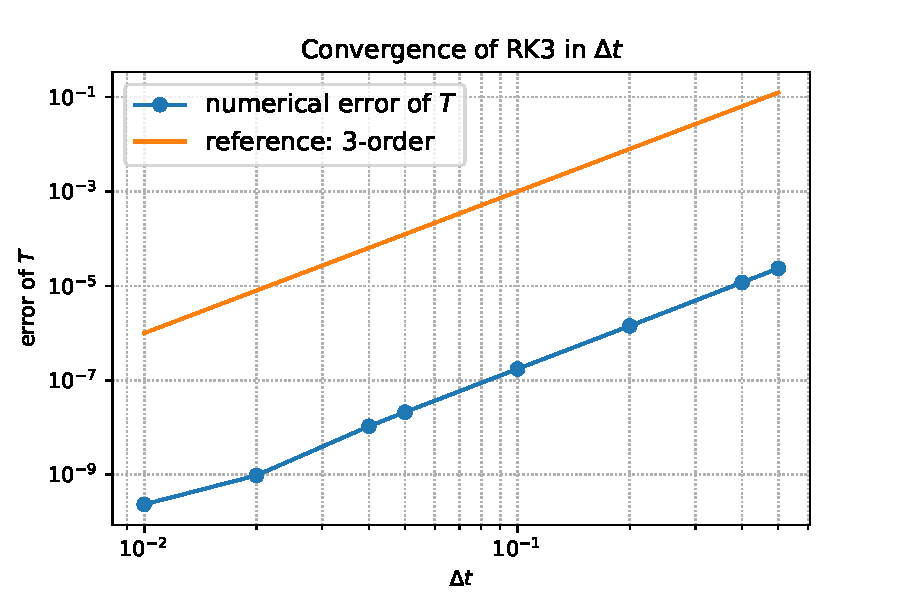
\includegraphics[width = .48\linewidth]{figs/sep/dt_2d_bkw_e=02}\hfill
%   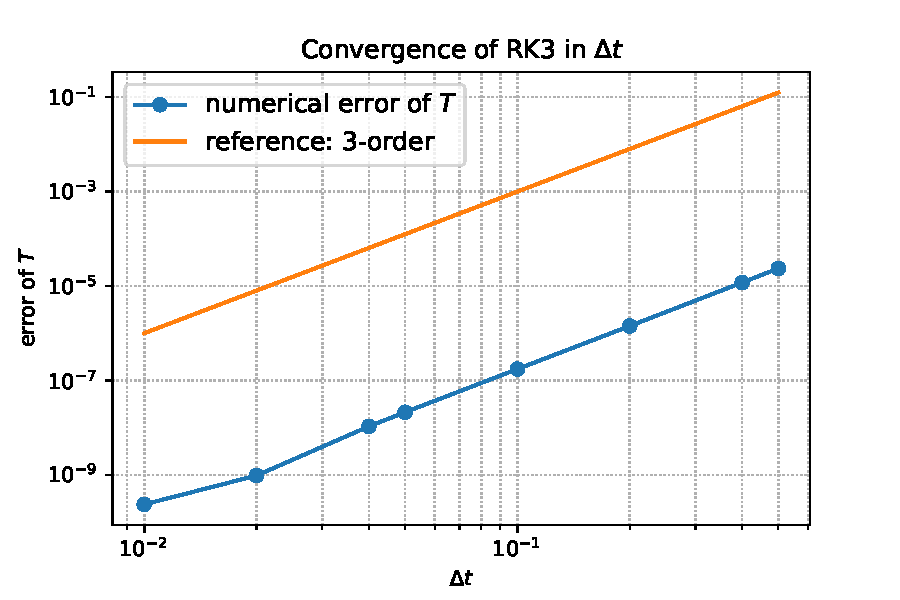
\includegraphics[width = .48\linewidth]{figs/full/dt_2d_bkw_e_full=02}
%   \caption{Convergence of RK3 with $e = 0.2$. Left: separate. Right: full.}
%   \label{dt_bkw_e02}
% \end{figure}
% \begin{figure}[htb]
%   \centering
%   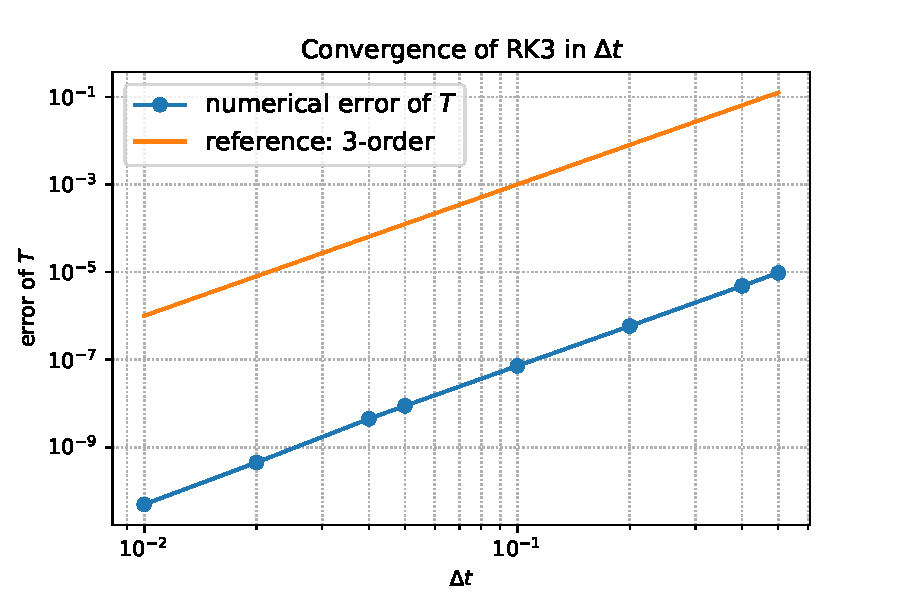
\includegraphics[width=0.5\textwidth]{figs/sep/dt_2d_bkw_e=05}\hfill
%   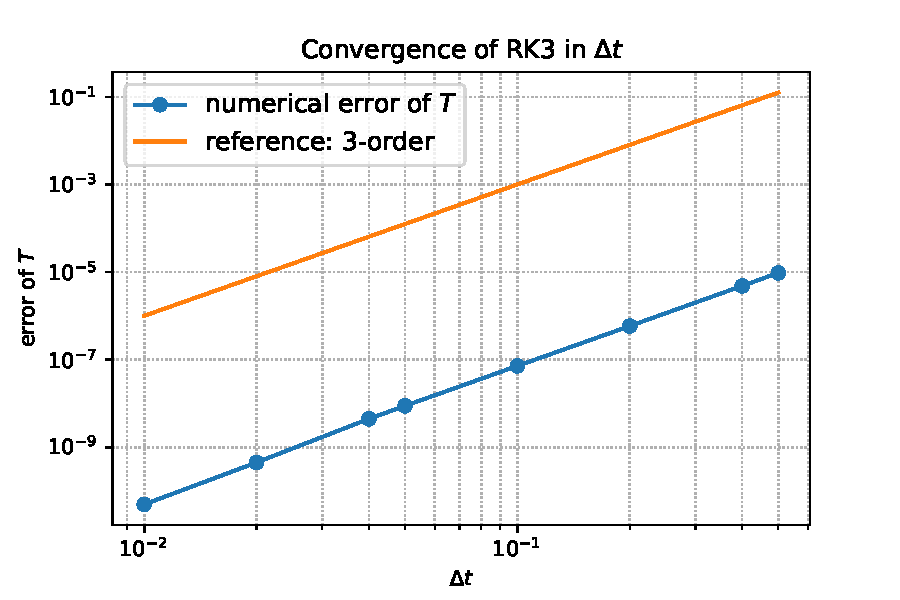
\includegraphics[width=0.5\textwidth]{figs/full/dt_2d_bkw_e_full=05}
%   \caption{Convergence of RK3 with $e = 0.5$. Left: separate. Right: full.}
%   \label{dt_bkw_e05}
% \end{figure}
% \begin{figure}[htb]
%   \centering
%   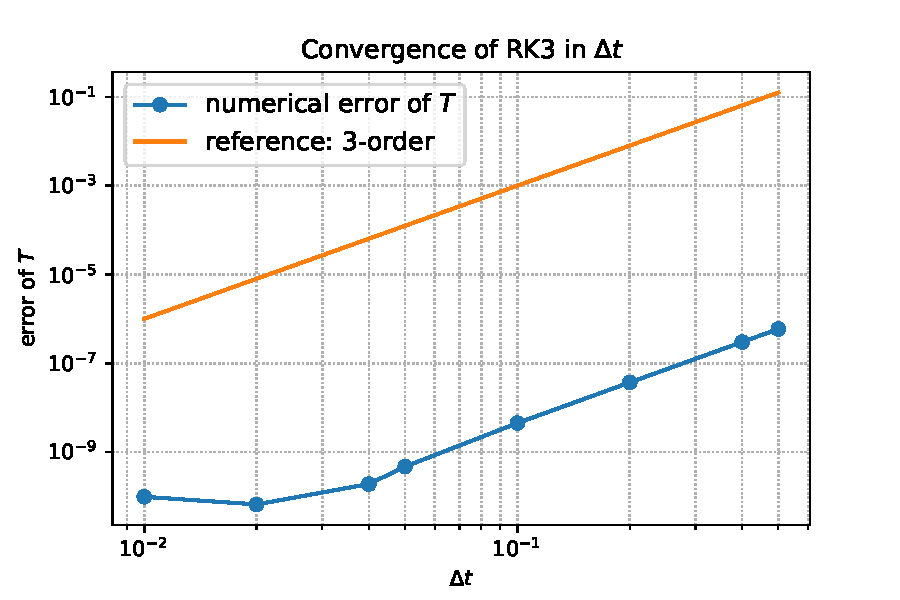
\includegraphics[width=0.5\textwidth]{figs/sep/dt_2d_bkw_e=08}\hfill
%   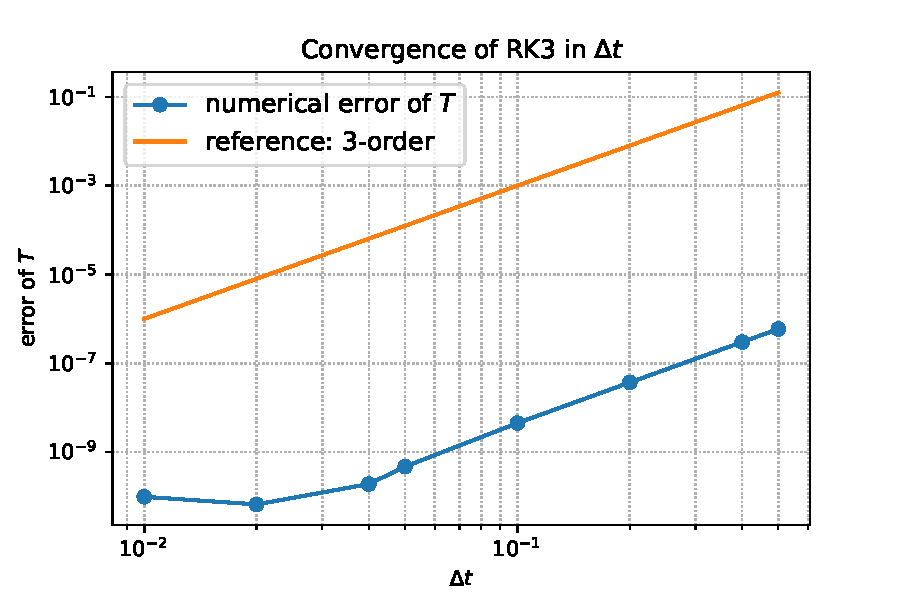
\includegraphics[width=0.5\textwidth]{figs/full/dt_2d_bkw_e_full=08}
%   \caption{Convergence of RK3 with $e = 0.8$. Left: separate. Right: full.}
%   \label{dt_bkw_e08}
% \end{figure}

\begin{figure}[htb]
  \centering
  \subfloat[$e = 0.2$, separate]{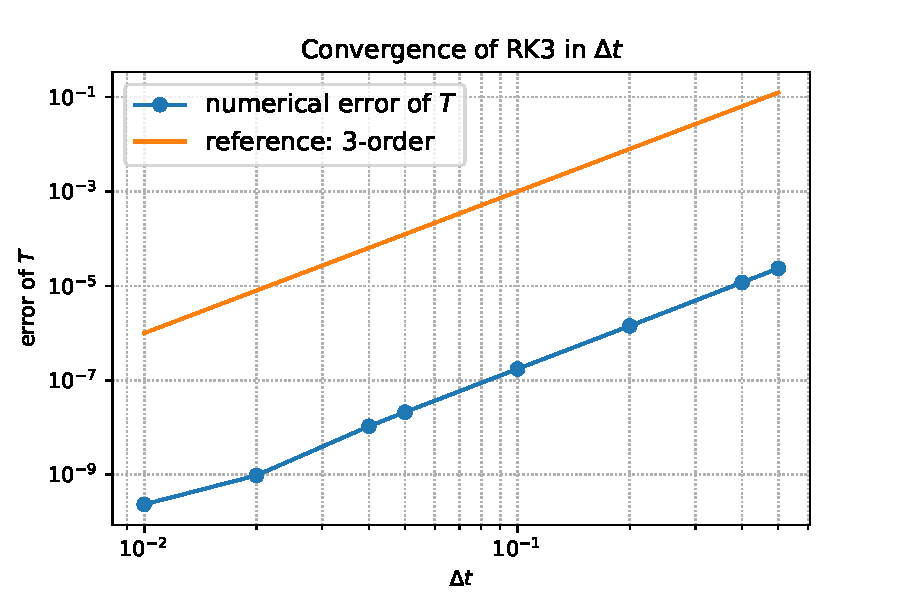
\includegraphics[width = 0.5\linewidth]{figs/sep/dt_2d_bkw_e=02}}\hfill
  \subfloat[$e = 0.2$, full]{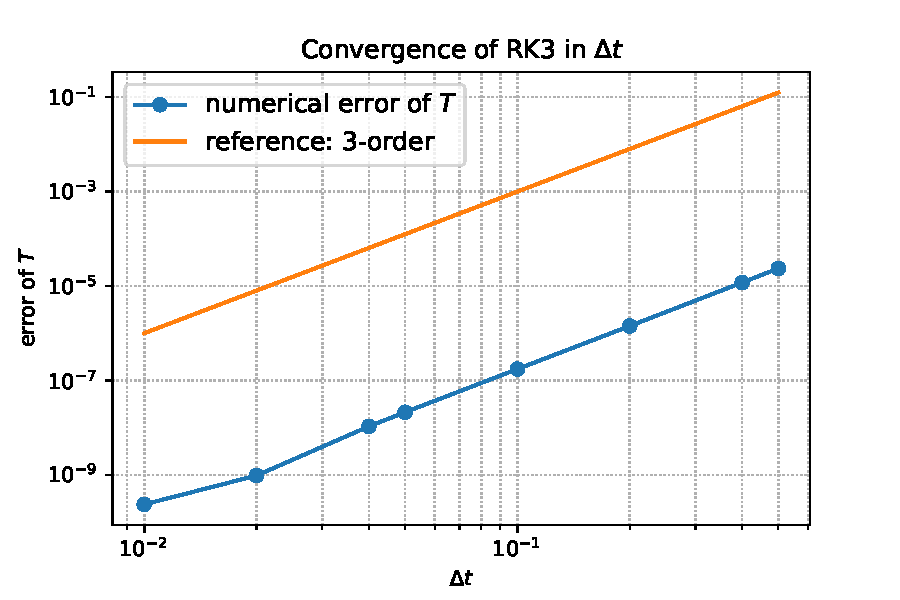
\includegraphics[width = 0.5\linewidth]{figs/full/dt_2d_bkw_e_full=02}} \\
  \subfloat[$e = 0.5$, separate]{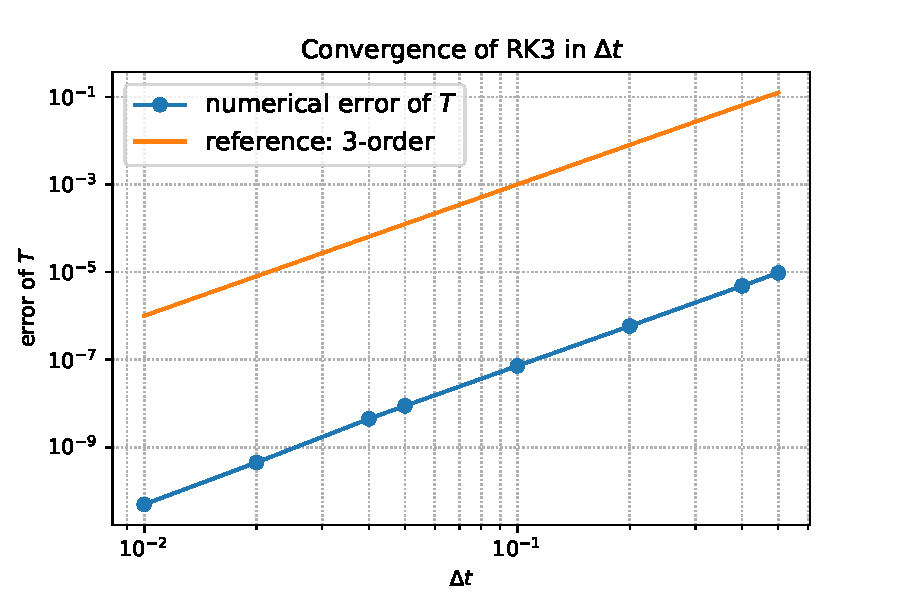
\includegraphics[width = 0.5\linewidth]{figs/sep/dt_2d_bkw_e=05}}\hfill
  \subfloat[$e = 0.5$, full]{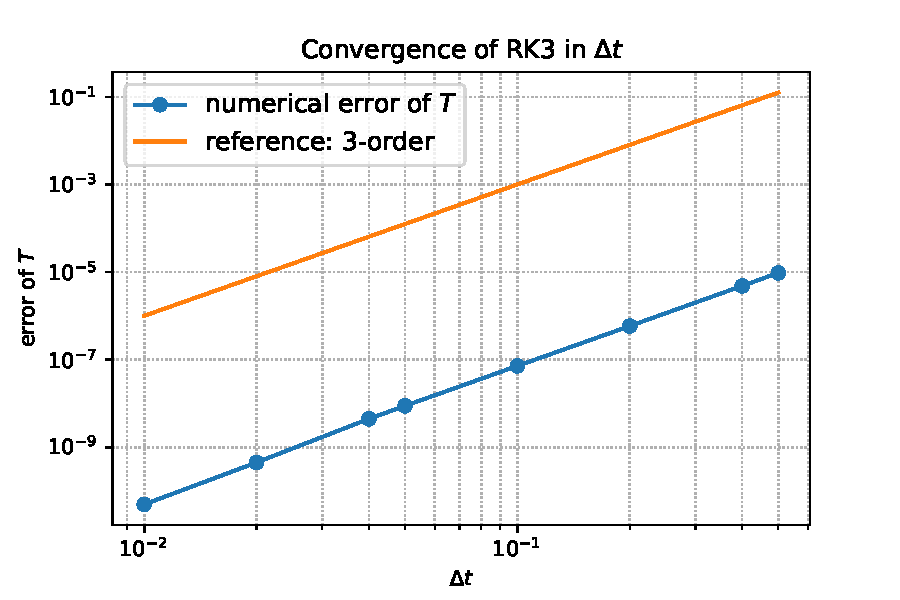
\includegraphics[width = 0.5\linewidth]{figs/full/dt_2d_bkw_e_full=05}} \\
  \subfloat[$e = 0.8$, separate]{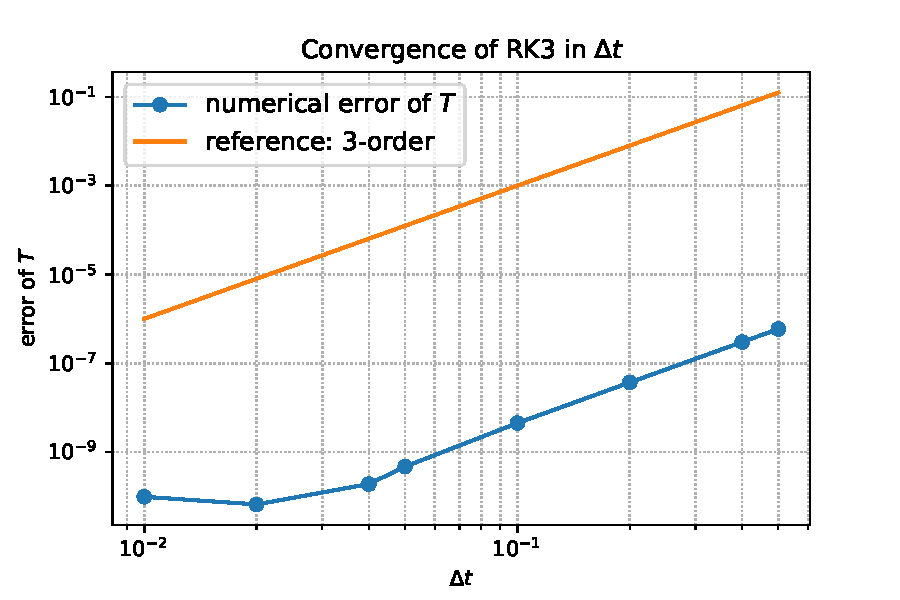
\includegraphics[width = 0.5\linewidth]{figs/sep/dt_2d_bkw_e=08}}\hfill
  \subfloat[$e = 0.8$, full]{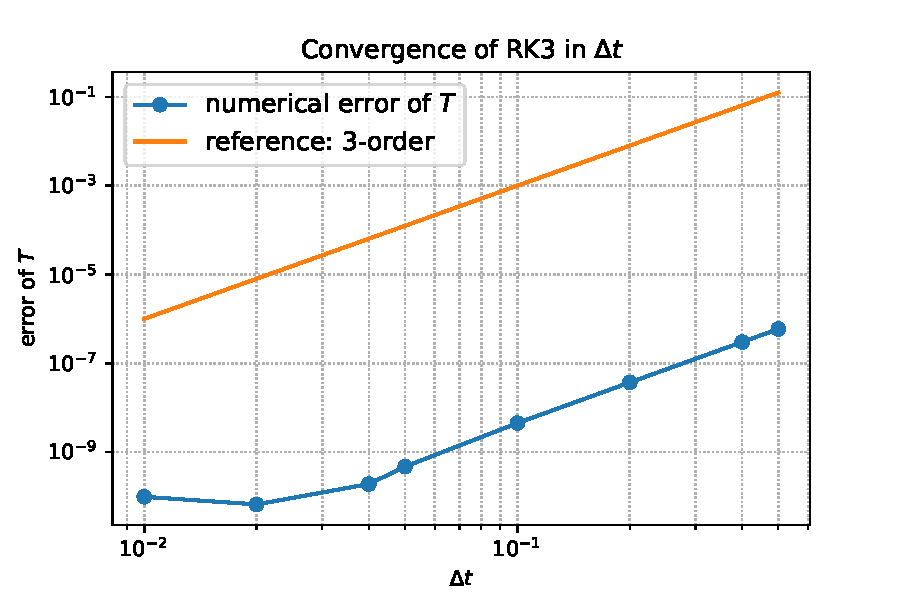
\includegraphics[width = 0.5\linewidth]{figs/full/dt_2d_bkw_e_full=08}}
  \caption{convergence in time 1}
  \label{dt_conv_1}
\end{figure}

\begin{figure}[htb]
  \centering
  \subfloat[$e = 0.2$, separate]{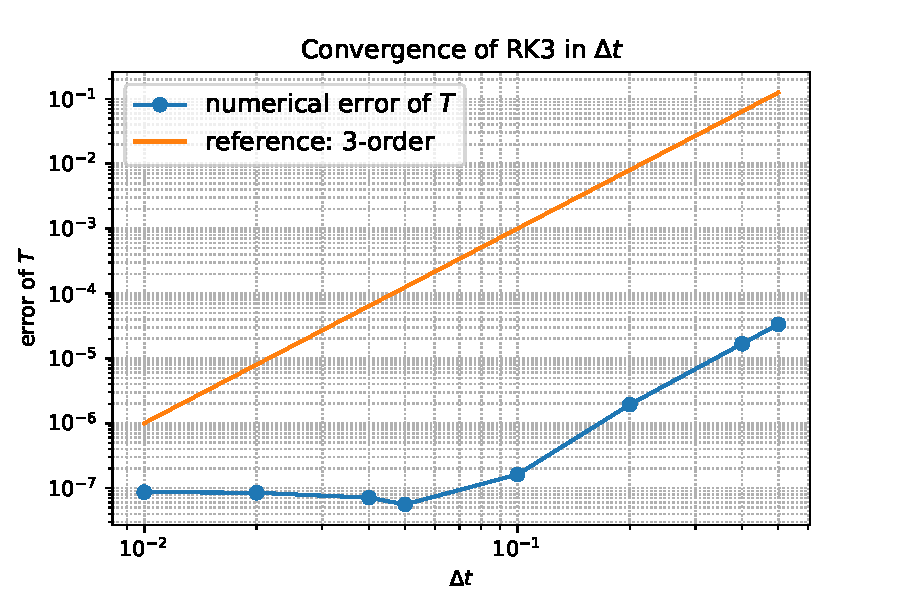
\includegraphics[width = 0.5\linewidth]{figs/sep/dt_2d_e=02}} \\
  \subfloat[$e = 0.5$, separate]{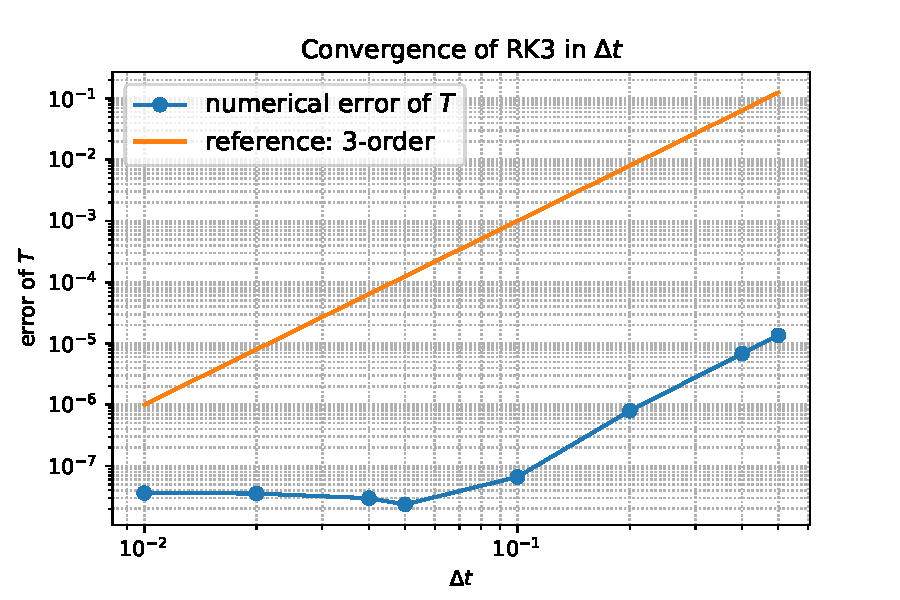
\includegraphics[width = 0.5\linewidth]{figs/sep/dt_2d_e=05}} \\
  \subfloat[$e = 0.8$, separate]{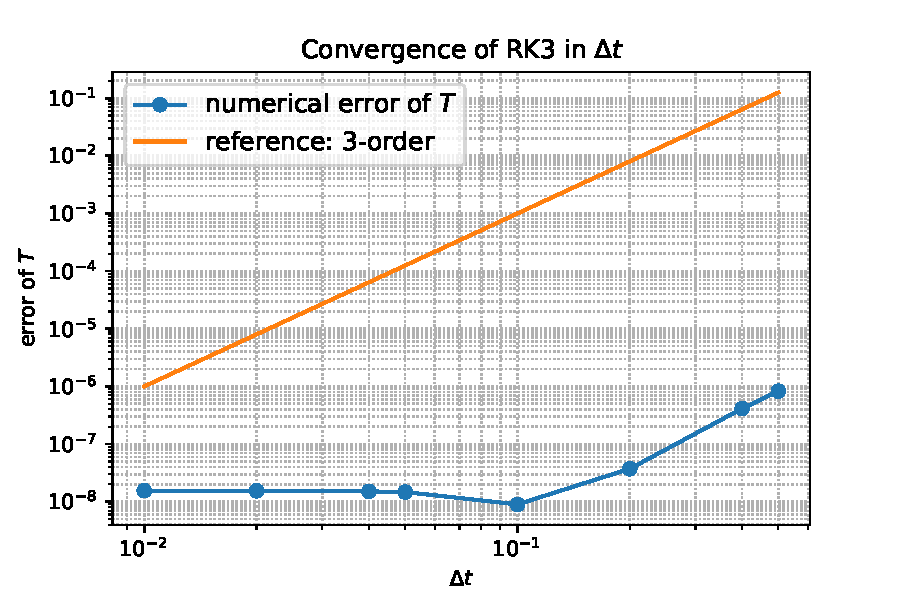
\includegraphics[width = 0.5\linewidth]{figs/sep/dt_2d_e=08}}
  \caption{convergence in time 2}
\end{figure}

This test shows that our RK3 method in time direction is indeed 3rd-order and in the following convergence tests of $N$ we will set $\Delta t = 0.01$

\paragraph{\bf Convergence in $N$} We then perform the convergence test of the spectral method. As mentioned previously we set $\Delta t = 0.01$ and $M = 30$, also $T_\text{final} = 2$. As $N$ increases from $8$ to $128$, we calculate the error for different $e$s using both "separate" and "full" method as shown in Table~\ref{N_bkw_e02}, Table~\ref{N_bkw_e05} and Table~\ref{N_bkw_e08}.

\begin{table}[htb]
  \centering
  \subfloat[$e = 0.2$]{
  \begin{tabu} to 0.6\linewidth {X[1, c] X[3, c] X[3, c]}
    \toprule
    $N$ & Separate & Full \\
    \midrule
    8 & 9.21116565e-01 & 9.21116565e-01 \\
    16 & 1.27634481e-02 & 1.27640374e-02 \\
    32 & 6.79544555e-06 & 6.79745658e-06 \\
    64 & 2.34851361e-10 & 2.36438646e-10 \\
    128 & 6.30565600e-11 & 6.13890050e-11 \\
    \bottomrule
  \end{tabu}
  } \\
  \subfloat[$e = 0.5$]{
  \begin{tabu} to 0.6\linewidth {X[1, c] X[3, c] X[3, c]}
    \toprule
    $N$ & Separate & Full \\
    \midrule
    8 & 7.98706096e-01 & 7.98706096e-01 \\
    16 & 6.42641236e-03 & 6.42644165e-03 \\
    32 & 4.55713801e-06 & 4.55730861e-06 \\
    64 & 4.93595165e-11 & 4.93770580e-11 \\
    128 & 3.13873372e-11 & 3.14279713e-11 \\
    \bottomrule
  \end{tabu}
  } \\
  \subfloat[$e = 0.8$]{
  \begin{tabu} to 0.6\linewidth {X[1, c] X[3, c] X[3, c]}
    \toprule
    $N$ & Separate & Full \\
    \midrule
    8 & 5.52666966e-01 & 5.52666966e-01 \\
    16 & 4.88821204e-04 & 4.88586534e-04 \\
    32 & 1.14430393e-07 & 1.13897201e-07 \\
    64 & 9.82359749e-11 & 9.82520731e-11 \\
    128 & 1.00099595e-10 & 1.00117470e-10 \\
    \bottomrule
  \end{tabu}
  }
  \caption{convergence in N 1}
  \label{table 1}
\end{table}

\begin{table}[htb]
  \centering
  \subfloat[$e = 0.2$]{
  \begin{tabu} to 0.6\linewidth {X[1, c] X[3, c] X[3, c]}
    \toprule
    $N$ & Separate & Full \\
    \midrule
    8 & 1.25303916e-01 & 1.25303916e-01 \\
    16 & 1.41601818e-02 & 1.42811856e-02 \\
    32 & 1.21162093e-04 & 8.50383206e-05 \\
    64 & 8.65618628e-08 & 5.75217760e-05 \\
    128 & 2.64749862e-08 & 5.74603408e-05 \\
    \bottomrule
  \end{tabu}
  } \\
  \subfloat[$e = 0.5$]{
  \begin{tabu} to 0.6\linewidth {X[1, c] X[3, c] X[3, c]}
    \toprule
    $N$ & Separate & Full \\
    \midrule
    8 & 9.06935081e-02 & 9.06935081e-02 \\
    16 & 2.06153352e-02 & 2.07345865e-02 \\
    32 & 1.08598123e-04 & 7.68575010e-05 \\
    64 & 3.61540865e-08 & 4.58166915e-05 \\
    128 & 4.84827622e-09 & 4.57852460e-05 \\
    \bottomrule
  \end{tabu}
  } \\
  \subfloat[$e = 0.8$]{
  \begin{tabu} to 0.6\linewidth {X[1, c] X[3, c] X[3, c]}
    \toprule
    $N$ & Separate & Full \\
    \midrule
    8 & 4.21932177e-02 & 4.21932177e-02 \\
    16 & 2.19257970e-02 & 2.17989934e-02 \\
    32 & 1.25546782e-04 & 1.17000137e-04 \\
    64 & 1.55334599e-08 & 2.42867607e-05 \\
    128 &  5.91159477e-09 & 2.42767854e-05 \\
    \bottomrule
  \end{tabu}
  }
  \caption{convergence in N 2}
  \label{table 2}
\end{table}




These results show that our method indeed can achieve spectral accuracy.



\subsection{3D example}

\paragraph{\bf Accuracy of spherical design}

\paragraph{\bf Haff's cooling law}
\begin{figure}[htb]
  \centering
  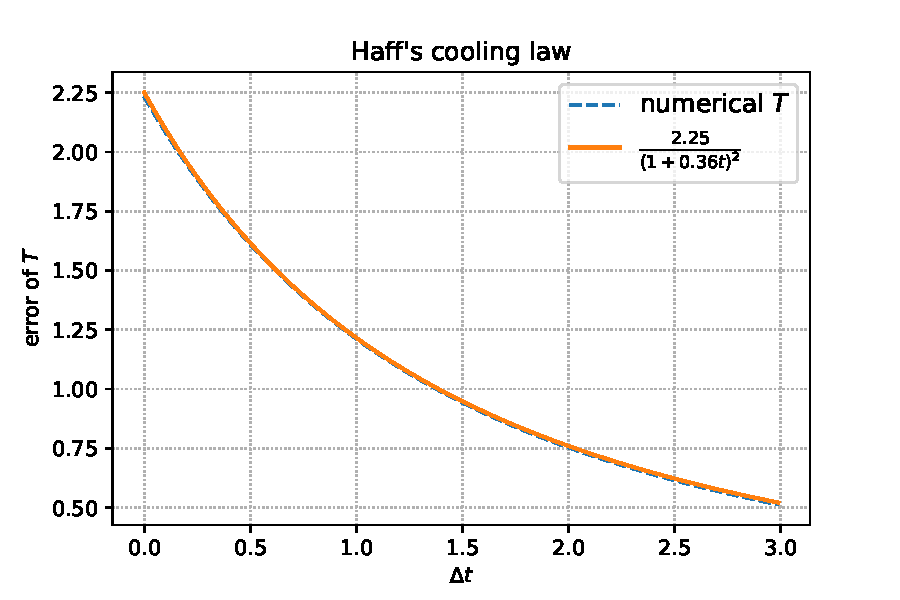
\includegraphics[width = .8\linewidth]{figs/Haff's_cooling}
  \caption{Haff's cooling law}
  \label{Haff_cooling}
\end{figure}


\section*{References}

% \bibliography{mybibfile}

\end{document}